% !TEX root = pfe-book3.tex
%!TEX TS-program = pdflatex
%!TEX encoding = UTF-8 Unicode


\cleardoublepage
%\mainmatter
\chapter{Summary of Electrical Engineering}
\label{ch-04}

\section{Sinusoidal EMF}

Storage batteries and dry batteries are sources of direct current. Electric power mains, on the other hand, provide us with alternating current. The words ``direct'' and ``alternating'' refer to the values of the voltage, emf and current. If these quantities remain unchanged as the current passes through a circuit, the current is said to he \emph{constant}, or \emph{direct (d-c)}; if they vary, the current is said to be \emph{alternating (a-c)}.

An electric current may vary in different ways with time in accordance with the device producing the current. The curve described by the change in electric current can be obtained by means of a cathode-, or electron-beam, tube. The electron ray is deflected by the fields of two mutually perpendicular parallel-plate capacitors. Applying various voltages across the capacitor plates, we can make the luminous spot produced by the ray wander all over the screen.

To obtain a picture of an alternating current, we proceed as follows. A so-called sawtooth voltage is applied across one pair of plates. The curve of this voltage is illustrated in \figr{fig-4.1}. If the electron beam is subject only to its action, the spot travels uniformly across the fluorescent screen and then returns with a jump to its starting point. The position of the spot provides information on the instant of time. When the alternating voltage being investigated is applied across the second pair of plates, the spot is given an up-and-down motion as it sweeps across the screen, producing a waving line in the same manner that mechanical vibrations could be made visible by a simple device as shown in Book~1. 
\begin{figure}[!ht]
\centering
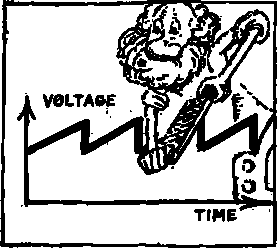
\includegraphics[width=0.4\textwidth]{figures/fig-04-01.pdf}
\caption{A graphical representation of varying voltage.}
\label{fig-4.1}
\end{figure}

It was no slip of the tongue when I mentioned ``vibrations'' (or ``oscillations''). Most of the quantities characterizing an alternating current oscillate according to the same harmonic or sine-curve law that a pendulum complies with when deviated from its equilibrium position. This can be readily shown by connecting \emph{a-c} city mains to an oscillograph.

Either the current or the voltage may be plotted along the vertical direction. The characteristics of the current are the same as parameters of mechanical vibrations. The interval of time after which the picture of current change is repeated is called the period $T$. Current frequency $\nu$, the reciprocal of the period, is usually equal to 50 or 60 cycles per second.

When we examine a single sine curve (as the curve obtained for alternating voltage or current is called), the selection of the initial instant of time is of no consequence. But if two sine curves are superimposed, as illustrated in \figr{fig-4.2}, we must specify the fraction of a cycle that they are shifted in phase. The phase is expressed by the angle $\varphi =2 \pi t/T$. Thus, if the curves are displaced with respect to each other by one-fourth of a period, we say they have a phase shift of \ang{90}; if by one-eighth of a period, the phase shift is \ang{45}, etc.

\begin{figure}[!ht]
\centering
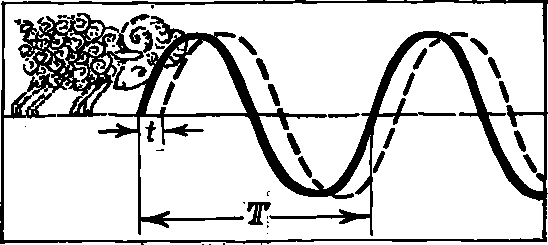
\includegraphics[width=\textwidth]{figures/fig-04-02.pdf}
\caption{The phase difference between two sine waves.}
\label{fig-4.2}
\end{figure}

When we are discussing several sine curves, shifted in phase, engineers speak of current or voltage vectors. The length of the vectors represents the amplitude of the sine curve, and the angle between them represents the phase shift. Many engineering devices provide a current whose curve is the sum of several sine curves displaced with respect to one another, rather than a simple sinusoidal current.

We shall show that a simple sinusoidal current is produced when the conducting loop rotates at constant speed in a uniform magnetic field.

Upon an arbitrary direction of the rectangular loop with respect to the lines of force, the magnetic flux passing through the loop equals
\begin{equation*}%
\Phi = \Phi_{\textrm{max}} \sin \varphi
\end{equation*}
where $\varphi$ is the angle between the plane of the loop and the direction of the field. This angle varies with the time according to the law $\varphi =2 \pi t/T$.

The law of electromagnetic induction enables us to calculate the induced emf. Let us write the equations of the magnetic fluxes for two instants, differing by the extremely small time interval $\tau$:
\begin{align*}%
\Phi & = \Phi_{\textrm{max}} \sin \frac{2\pi}{T} \, t \qq{and} \\
\Phi & = \Phi_{\textrm{max}} \sin \frac{2\pi}{T} \, (t + \tau) 
\end{align*}
The difference between these two equations is
\begin{align*}%
2 \Phi_{\textrm{max}} \cos \frac{2 \pi}{T}\left( t + \frac{\tau}{2} \right) \sin \left( \frac{2 \pi}{T} \frac{\tau}{2} \right) 
\end{align*}
Since $\tau$ is very small, the following approximate equations are valid:
\begin{align*}%
\sin \left( \frac{2 \pi}{T} \frac{\tau}{2} \right)  & \approx \frac{2 \pi}{T} \frac{\tau}{2} \qq{and} \\
\cos \frac{2 \pi}{T}  \, (t + \tau)  & \approx \cos \frac{2 \pi}{T} t
\end{align*}
The induced emf is equal to this difference referred to the time. Then
\begin{align*}%
\mathcal{E}^{\textrm{ind}} & = \frac{2 \pi}{T}\, \Phi_{\textrm{max}} \cos \frac{2 \pi}{T} \, t \\
& = \frac{2 \pi}{T}\, \Phi_{\textrm{max}} \sin \left(\frac{2 \pi}{T} \, t - \frac{\pi}{2} \right)
\end{align*}
We have shown that the induced emf is expressed by a sine curve shifted in phase with respect to magnetic flux sine curve by \ang{90}. As for the maximum value of induced emf, its amplitude, it is proportional to the product of the magnetic flux amplitude by the frequency of rectangular loop rotation.

The law for the current is obtained by dividing the induced emf by the resistance of the circuit. But we shall make a crude error if we equate the resistance to alternating current, in the denominator of the equation
\begin{equation*}%
I_{\textrm{ac}} = \frac{\mathcal{E}^{\textrm{ind}}}{R_{\textrm{ac}}}
\end{equation*}
to the ohmic resistance, i.e. the quantity we have dealt with previously. It turns out that $R_{\textrm{ac}}$ is determined not only by the ohmic resistance hut also by two more parameters of the circuit: its inductance and the capacitances connected into the circuit.
\begin{figure}[!ht]
\centering
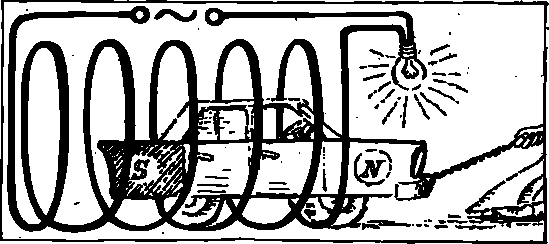
\includegraphics[width=\textwidth]{figures/fig-04-03.pdf}
\caption{Effect of an iron core in a circuit.}
\label{fig-4.3}
\end{figure}

The fact that Ohm's law is more complicated for alternating current than for direct current is demonstrated by the following simple experiment. Illustrated in \figr{fig-4.3} is an electric circuit with the current passing through an electric lamp and a coil into which an iron core can be inserted. First we connect the lamp circuit to a \emph{d-c} source. Next we move the core into the coil and pull it out. No effect whatsoever! The resistance of the circuit remains constant and so does the current. We repeat the experiment for the case when the circuit is connected to an \emph{a-c} source. The result is spectacular, is it not? Now the lamp burns brightly when the core is not inserted into the coil, and gradually dims as it is inserted.

Thus, at a constant external voltage, and a constant ohmic resistance (depending only on the material, length and cross section of the wire), the current varies with the position of the iron core in the coil.

What does this mean?

Recall that an iron core drastically increases the magnetic flux passing through the coil (by thousands of times). For an alternating current, the flux varies continually. But if it varied without the iron core from zero to some arbitrary unit, with the core it varies from zero to several thousand units.

As the magnetic flux varies, the lines of force thread through the turns of their ``own'' coil. This produces a current of self-induction in the coil. According to Lenz's law, the induced current is in the direction that weakens the effect that causes it: the external emf meets with an obstacle that did not exist when the current was direct. In other words, an alternating current is subject to an additional resistance because the magnetic field, threading through the wires of its own circuit, produces a back electromotive force, called the \emph{emf of self-induction}, which weakens the average current. This additional resistance is called \emph{inductive reactance}, to distinguish it from a true (ohmic) resistance.

Experiments indicate (and this will seem quite natural to the reader) that the magnetic flux threading through the coil (or, more generally speaking, the whole
current-carrying circuit) is proportional to the current: $\Phi = LI$. As for the proportionality factor $L$, called the \emph{inductance}, it depends upon the geometry of the circuit or coil and what kind of cores it encompasses. As is obvious from the formula, the numerical value of the inductance is equal to the magnetic flux when the current equals one ampere. The unit of measurement of $L$ is the \emph{henry} $(\SI{1}{\henry}= \SI{1}{\ohm\second})$.

We can theoretically derive and prove by experiments that the inductive reactance $R_{L}$ is expressed by the formula
\begin{equation*}%
R_{L} = 2\pi \nu L
\end{equation*}
If the ohmic resistance (with which we are already acquainted) and the capacitive reactance (which we shall discuss below) are small, the current in an \emph{a-c} circuit equals
\begin{equation*}%
I = \frac{\mathcal{E}}{R_{L}}
\end{equation*}
To be able to judge what is meant by ``small'' or ``large'', we can calculate the inductive reactance for the frequency of ordinary city power supply current and an inductance of \SI{0.1}{\henry}. We obtain about \SI{30}{\ohm}.

Now, what would a coil with an inductance of one henry be like? The following formula, which we give without derivation, is used to assess the inductance of coils and chokes (coils with an iron core):
\begin{equation*}%
L= \mu_{0}\mu \frac{n^{2}}{l}A \qq{and} \mu_{0} = 4\pi \times \num{d-7} \si{\joule\per\ampere\squared\per\meter}
\end{equation*}
where $n$ = number of turns; $l$ = length of the coil; and $A$ = cross-sectional area. Thus, an inductance of \SI{0.002}{\henry} can be obtained, for instance, with a coil having the following parameters: $l = \SI{15}{\centi\meter}$, $n = 1500$ and $A = \SI{1}{\centi\meter\squared}$. If an iron core with $\mu = 1000$ is inserted into this coil, its inductance equals 2 henries.

An emf of any origin and, consequently, an emf of self-induction, performs work. This work, as we know, is equal to $\mathcal{E}I$. If the current is alternating, the values of $\mathcal{E}$ and $I$ vary each instant. Let their values equal $\mathcal{E}_{1}$ and $I_{1}$ at the instant $t$ and $\mathcal{E}_{2}$ and $I_{2}$ at the instant $(t+ \tau)$. The magnetic flux threading the turns of a coil of inductance $L$ is equal to $LI$. At the instant $t$, its value
is $LI_{1}$ and at the instant $(t+\tau)$, it is $LI_{2}$. What amount of work is required to increase the current from $I_{1}$ to $I_{2}$. The emf is equal to the change in magnetic flux divided by the time during which the change took place:
\begin{equation*}%
\mathcal{E} = \frac{L(I_{2} - I_{1})}{\tau}
\end{equation*}
This equation is to be multiplied by the time and the current, i.e. $\mathcal{E}I\tau$, to obtain the amount of work. But by what current? The average value: $(I_{1}+I_{2})/2$. Hence, the work of the emf of self-induction equals 
\begin{equation*}%
\frac{L}{2}\, (I_{2}+I_{1})\, (I_{2} - I_{1}) = \frac{L}{2} \,I_{2}^{2} - \frac{L}{2} \,I_{1}^{2}
\end{equation*}
This arithmetical result can be expressed in words: the work performed by the emf equals the difference in the values of $LI^{2}/2$ at two instants of time. This means that energy is not dissipated by an inductive reactance; it is not converted into heat as in circuits with ohmic resistance, but is transferred into the ``reserve''. For this reason, we can rightly call the quantity $LI^{2}/2$, the \emph{magnetic energy of the current}.

Now let us discuss the effect of introducing a capacitor into an alternating current circuit.

If we include a capacitor in a \emph{d-c} circuit, there is no current. Introducing a capacitor is the same thing as breaking the circuit. But the current is not interrupted by a capacitor in an \emph{a-c} circuit.

The difference is what interests us; what is it? The explanation is simple enough. When the circuit is connected to an \emph{a-c} power source, an electric charge begins to accumulate on the plates of the capacitor. The positive charge goes to one plate and negative to the other. Assume that the inductive reactance and ohmic resistance are low. Charging continues until the voltage across the capacitor plates reaches a maximum and is equal to the emf of the power source. At this instant, the current equals zero. Then the voltage of the source begins to drop and the capacitor is ``discharged''.

If we measure the current with some instrument in a circuit containing a capacitor, we shall find that the current varies in accordance with two quantities. In the first place, it can be proved (both by experiments and by theoretical reasoning) that the current decreases with the frequency. This means that the \emph{capacitive reactance} is inversely proportional to the frequency. This result is quite natural because the lower the frequency, the more alternating current, so to speak, approximates direct current.

If we change the geometrical parameters of the capacitor, i.e. the distance between the plates and their area, we shall find that the capacitive reactance is also inversely proportional to the capacitance of the capacitor.

The formula for capacitive reactance is of the form: 
\begin{equation*}%
R_{C}= \frac{1}{2\pi \nu C}
\end{equation*}
At the frequency of city power supply current, i.e, 50 cps (cycles per second), a capacitor with a capacitance of \SI{30}{\micro\farad} constitutes a capacitive reactance of about \SI{100}{\ohm}.

I do not intend to relate how the total resistance (called the \emph{impedance}) is calculated in complex circuits consisting of ohmic resistances, and inductive and capacitive reactances. I only wish to warn the reader that the impedance is not the sum of the separate resistances and reactances.

The electric current in a part of a circuit that includes an ohmic resistance, a capacitor and an inductive coil, and the voltage across this part can be measured in the ordinary way by means of an oscilloscope (electron- beam tube). We see both the current and the voltage on the screen in the form of sine curves. It should not surprise us to find that these sine curves are shifted with respect to each other by a certain phase angle $\varphi$. (The reader readily comprehends that this must be so if he recalls that, for instance, the current equals zero in a circuit with a capacitor when the voltage across the capacitor reaches its maximum value.)

The value of the phase shift $\varphi$ is of prime importance.

The power transmitted equals the product of the current by the voltage. If the current and voltage sine curves coincide, the power has its maximum value. But if they are shifted as they would be in a circuit including only capacitive or only inductive reactance, the power equals zero. This can easily be demonstrated by plotting two sine curves with a phase shift of \ang{90}, multiplying their ordinates together at each point and adding together these products over a single period. It can be strictly demonstrated that the average power per period of alternating current equals
\begin{equation*}%
P = IV \cos \varphi
\end{equation*}
One of the main concerns of the electrical engineer
is to increase $\cos \varphi$ (called the \emph{power factor}). 

\section{Transformers}

You have just purchased an electric refrigerator. The salesperson warned you that the refrigerator is designed for a mains voltage of \SI{220}{\volt}. But in your home the mains voltage is \SI{127}{\volt}. Is this a hopeless situation? Not at all. You must simply spend a little more and buy a suitable transformer.

A \emph{transformer} is a very simple device enabling you to either raise or lower the voltage. It consists of a laminated iron core on which two coils have been wound. Each coil, or winding, has a different number of turns.

When we plug one of the windings into a socket with the mains voltage, we find with a voltmeter that the voltage across the ends of the second winding differs from that of the power mains. If the primary winding has $w_{1}$ turns and the secondary, $w_{2}$ turns, the ratio of the voltages is
\begin{equation*}%
\frac{V_{1}}{V_{2}} = \frac{w_{1}}{w_{2}} 
\end{equation*}
Thus, a transformer steps up the voltage when the primary voltage is connected to the winding with the smaller number of turns, and steps down the voltage in the opposite case.

Why is this so? The fact is that practically the whole magnetic flux is within the iron core. This means that both windings are linked by an equal number of lines of force. A transformer can operate only with an alternating voltage across the primary winding. A sinusoidal current variation in the primary winding induces a sinusoidal emf in the secondary winding. Each turn of the primary and secondary windings are in identical conditions. The emf per turn of the primary winding is equal to the emf of the power mains divided by the number of turns of the primary winding, i.e. $V_{1}/w_{1}$, and the emf of the secondary winding is equal to the product of $V_{1}/w_{1}$ by the number $w_{2}$ of turns of the secondary winding.

In principle, each transformer can be employed either as a step-up or a step-down device depending upon the winding to which the primary voltage is applied.

\begin{figure}[!ht]
\centering
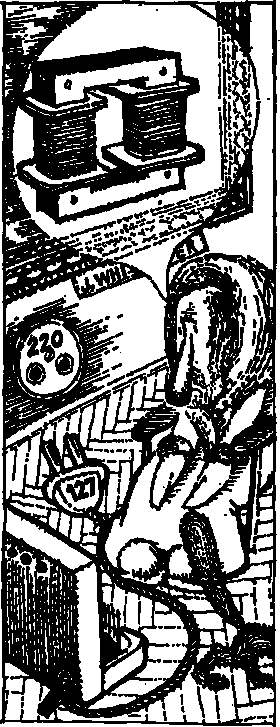
\includegraphics[width=0.4\textwidth]{figures/fig-04-04.pdf}
\caption{A transformer in action changes the input voltage to a desirable value.}
\label{fig-4.4}
\end{figure}


One frequently deals with transformers in everyday life (\figr{fig-4.4}). Besides the transformers we employ willy-nilly because some electric appliance is designed for one voltage and the city mains for another, we may also have to deal with the spark coil of an automobile. The spark coil is a step-up transformer. To produce the sparks that ignite the fuel mixture in the cylinders, we require a high voltage. It is obtained from the storage battery of the automobile, after converting its direct current into alternating current by means of an interrupter (contact-breaker) and then stepping up the voltage with a spark coil.

It can readily be seen that when the voltage is stepped up, the current is reduced and vice versa, with an accuracy within the energy losses due to the heating of
the transformer.

Welding apparatus requires step-down transformers. An exceptionally heavy current is required for welding operations, and the transformer has only a single output turn.

You have probably noted that the core of a transformer is made of thin sheets of steel. This is done to prevent energy losses in converting voltages. As mentioned previously, eddy currents have a considerably weaker effect on sheet stock than on solid material.

In the home you deal with small low-power transformers. Powerful transformers are huge structures. In them the core with tts windings is inserted into a tank filled with cooling oil.

\section[Machines that Produce Electric Current]{Machines that Produce \\Electric Current}

Machines that convert mechanical motion into electric current were first developed only some hundred and fifty years ago.

The first generator of electric current was the machine built by Michael Faraday and consisted of a rectangular loop of wire rotating in a field set up by permanent magnets. Soon somebody (but not Faraday) got the idea of replacing the single loop with a whole coil, thereby adding all the emf induced in all the turns. Only in 1851 were the permanent magnets replaced by electromagnets, i.e. coils wound on an iron core. Originated with these devices was the expression ``exciting the machine'' because it was necessary first to ``vitalize'' the electromagnet before an electric current could be produced. The early generators were separately excited from some outside power source.

The next stage in generator development was the discovery of the principle of self-excitation, which eliminated the necessity of a separate power supply to excite the electromagnets. It proved sufficient to connect the excitation, or field, winding of the generator in some manner to the main winding. By the end of the eighties of last century, electric machines had already acquired the principal features they have today. The simplest model of a \emph{d-c} generator is illustrated in \figr{fig-4.5}. If the loop is rotated in a field of permanent magnets, a sinusoidal emf is induced in it.

\begin{figure}[!h]
\centering
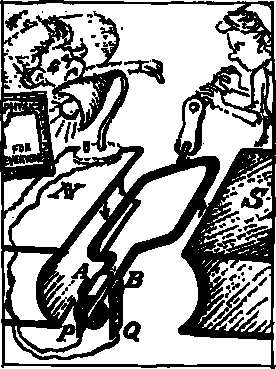
\includegraphics[width=0.45\textwidth]{figures/fig-04-05.pdf}
\caption{A simple \emph{d-c} generator.}
\label{fig-4.5}
\end{figure}


If you wish to obtain a direct current from the alternating current in the loop, it will be necessary to equip the generator with a special device called a split-ring commutator. This commutator consists of two half-rings, $A$ and $B$, insulated from each other and mounted on a common cylinder (see \figr{fig-4.5}). This cylinder rotates together with the rectangular loop. Applied to the half-rings are contacts $P$ and $Q$ (called brushes), by means of which the current is conducted to the external circuit. Upon each half-revolution of the loop, its commutator half-rings pass from one brush to the other. Hence, notwithstanding the reversal of the current in the loop itself, the current in the external circuit has only a single direction. Since the rotating component (rotor) of a real machine consists of a great number of loops, or sections, displaced through a definite angle with respect to one another, and the commutator consists of the corresponding number of segments, we obtain a practically constant emf.

%\newpage
\begin{center}
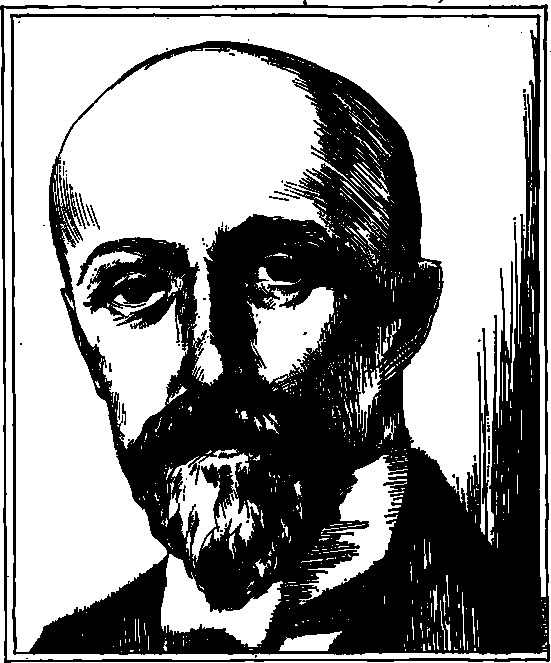
\includegraphics[width=0.8\textwidth]{figures/dobrovosky.pdf}
\end{center}
{\small \textsf{{Mikhail Osipovich Dolivo-Dobrovolsky [1862-1919]}} -- \textsf{\footnotesize distinguished Russian scientist and engineer; he developed the three-phase current systems, which are the foundation of all modem electrical engineering. He worked out all the elements of three-phase circuits with alternating currents. In 1888 he built the first three-phase \emph{a-c} generator with a rotating magnetic field.}}


\emph{D-c} generators are being built today with a power rating from fractions of a kilowatt to several thousand kilowatts. Powerful generators are employed for the power supply in electrolysis in the chemical industry and in nonferrous metallurgy (aluminium and zinc production). They are designed for a large current and a relatively low voltage (120 to \SI{200}{\volt} and 1000 to \SI{20000}{\ampere}). \emph{D-c} generators are likewise used for electric welding.


But \emph{d-c} generators are not the main producers of electric power. Alternating current with a frequency of \SI{50}{\hertz} (or cps) is applied in the USSR for the production and distribution of electric energy. An \emph{a-c} generator, called an alternator, is designed so that it simultaneously produces three emf's of the same frequency, differing in phase by the angle $2\pi/3$.

\begin{figure}[!ht]
\centering
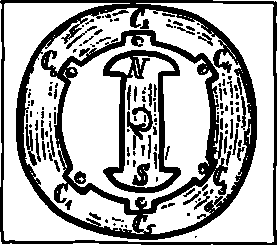
\includegraphics[width=0.4\textwidth]{figures/fig-04-06.pdf}
\caption{A schematic of a three phase generator.}
\label{fig-4.6}
\end{figure}

Such a three-phase generator is shown schematically in \figr{fig-4.6}. In the drawing each coil is represented by a single turn. The wire of one turn is denoted by $C_{1}$-$C_{4}$; the second, $C_{2}$-$C_{5}$ and the third, $C_{3}$-$C_{6}$. If the current enters $C_{1}$, it returns through $C_{4}$, etc. (Of course, at instants corresponding to various relative positions of the rotor and stator, any of these leads, or wires, may be points of entry or exit of the current.) The emf in the stationary turns of the stator is induced because they cut across the magnetic field of the rotating electromagnet, the rotor. As the rotor rotates at constant speed, a periodically varying emf is induced in the windings of each phase of the stator. The three induced emf's are of the same frequency and differ from one another in phase by the angle \ang{120} as a result of their spatial displacement. 

The three turns of the winding can be either \emph{star} or \emph{delta connected}. These circuits were worked out and put into operation in the nineties of last century by Mikhail Osipovich Dolivo-Dobrovols-ky (1862-1919). In a star connection, the ends of all three windings of the generator stator, $C_{4}$, $C_{5}$ and $C_{6}$, are connected together at a single point, which is called the neutral, or zero, point. Four leads connect the generator to the consumer of the energy: three line wires, from the starts of the windings, $C_{1}$, $C_{2}$ and $C_{3}$ and a neutral wire from the neutral point of the generator. This is called a \emph{four-wire system}.

The voltage between the neutral point and the start of a phase is called the \emph{phase voltage}. The voltage between the starts of the windings is called the \emph{line voltage. These} voltages are related by the equation
\begin{equation*}%
V_{I} = \sqrt{3} \, V_{\textrm{ph}}
\end{equation*}
If the loads ($I$, $II$ and $III$) in the three phases are the same, the current in the neutral wire equals zero. In this case, the neutral wire can be done away with, using what is called a \emph{three-wire system}. Diagrams of star connections are illustrated in \figr{fig-4.7}.

\begin{figure}[!ht]
\centering
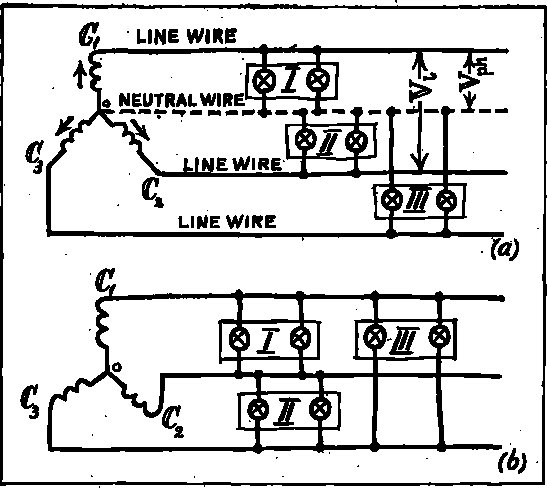
\includegraphics[width=\textwidth]{figures/fig-04-07.pdf}
\caption{A schematic of a star connection in a generator.}
\label{fig-4.7}
\end{figure}

A delta connection also allows a three-wire system to be employed. Here the end of each winding is connected to the start of the next one so that the windings form a closed triangle. The line wires are connected to the vertices of this triangle. Here the line voltage equals the phase voltage and the currents are related by the equation
\begin{equation*}%
I_{I} = \sqrt{3} \, I_{\textrm{ph}}
\end{equation*}
Three-phase circuits have the following advantages: more economical energy transmission than in single-phase circuits, and the feasibility of obtaining two voltages -- phase and line -- from a single installation.


The \emph{a-c} generator, or alternator, described above belongs to the class of synchronous machines. These are machines in which the speed of rotor rotation coincides with the speed of rotation of the magnetic field set up by the stator. Synchronous generators are the main producers of electric energy. They exist in several design versions, depending on the method of driving the rotor.

The reader may ask: If certain machines are said to be synchronous, are there asynchronous machines as well? Yes, there are! But they are employed as motors and we shall discuss them in the next section. There we shall also consider why the magnetic field rotates in a three-phase \emph{a-c} machine.

\section{Electric Motors}

More than half of all the electric energy produced is converted by electric motors into mechanical energy to satisfy the needs of industry, agriculture, transportation and the household. The most extensively used is the simple, reliable, inexpensive, easily maintained asynchronous, or induction, electric motor, invented in 1889 by the same talented Russian engineer Dolivo-Dobrovolsky. Its main features have been retained up to the present time. Motors of this type are used for the drives of various machine tools, pump and compressor installations, forging and pressworking machinery, materials handling and transportation equipment and other mechanisms.

The prototype of the induction motor was the model devised by the French physicist Dominique Francois Jean Arago (1786-1853). In 1824, Arago demonstrated before the Paris Academy of Sciences a phenomenon which he called ``magnetism of rotation''. He showed that a magnetic needle suspended over a rotating copper disk rotates with the:disk. The inverse is also true: a disk mounted on a pivot rotates if it is in the field of a rotating permanent magnet. This idea was brilliantly utilized by Dolivo-Dobrovolsky, who combined it with the features of a three-phase system of currents. This enabled rotation of the magnetic field to be obtained without using any additional devices.

Let us examine the schematic diagrams in \figr{fig-4.8}. For the sake of extreme simplification only three turns are shown (actually, of course, electric machines have windings with a great number of turns). The cross and black dot indicate whether the current flows away from us or toward us in each turn at a definite instant of time.
\begin{figure}[!ht]
\centering
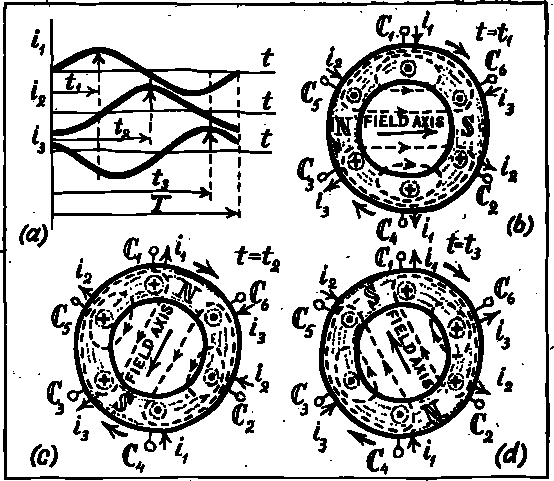
\includegraphics[width=\textwidth]{figures/fig-04-08.pdf}
\caption{Schematic diagram of a three-phase electric motor and its operation.}
\label{fig-4.8}
\end{figure}

The three turns make angles of \ang{120} with one another. \figr{fig-4.8}~\hlgray{(a)} shows the phase relations of the three currents $i_{1}$, $i_{2}$ and $i_{3}$ flowing in the turns. Of interest to us is the resultant magnetic field set up by the three ``coils''. \figr{fig-4.8}~\hlgray{(b)} shows the lines of force of the resultant field for instant $t_{1}$ (current flowing into $C_{2}$, $C_{3}$ and $C_{4}$). Similar diagrams are shown in \figr{fig-4.8}~\hlgray{(c)} and \hlgray{(d)} for instants $t_{2}$ and $t_{3}$ Hence, as we can see, the field we are interested in rotates (note the positions of the crosses), and rotates in the full sense of the word! The axis of the field in the middle of the system is aligned along the axis of the turn (phase) in which the current is maximum at the given instant of time.

\begin{figure}[!ht]
\centering
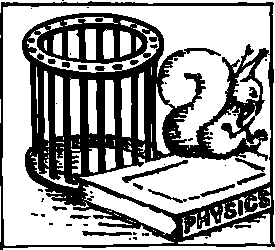
\includegraphics[width=0.5\textwidth]{figures/fig-04-09.pdf}
\caption{Armature for starting an \emph{a-c} motor.}
\label{fig-4.9}
\end{figure}

The diagrams we have just discussed give an idea of how a three-phase \emph{a-c} winding is arranged in the stator of a three-phase induction (asynchronous) electric motor. The rotor (\figr{fig-4.9}), set into motion by the rotating magnetic field, is short-circuited, i.e. we see neither the start nor the end of the winding. Such a rotor, also called an armature, resembles a squirrel cage. It consists of copper bars joining two copper rings. Compare it with a \emph{d-c} electric machine. How much simpler this is! We need only to connect a three-phase \emph{a-c} power supply to the stator. This sets up a rotating magnetic field in the machine. 

The magnetic lines of force of this field link the rods of the rotor, inducing currents in the rods and giving the motors their common name. As a result of the interaction between the rods, along which currents flow, and the magnetic field, the rotor begins to rotate at a speed near to that of the field, but does not reach this speed. This is just as needs be as otherwise the rods of the rotor would not cut the magnetic lines of force of the rotating field of the stator, and the rotor would stop. This is why such machines are said to be asynchronous. The lag of the rotor is called slip.

Induction electric motors are available in a large power range: from fractions of a watt to hundreds of kilowatts. There are even more powerful induction motors: up to \SI{6000}{\kilo\watt}, operating on a voltage of \SI{6000}{\volt}.

Asynchronous micromachines are used in automatic control systems as actuating mechanisms, or power units, to convert the input electric signal into mechanical motion of a shaft. They can also be used as tachogenerators for converting rotation into an electric signal.

The synchronous machines previously considered and \emph{d-c} machines can also be electric motors. This follows from the obvious principle of convertibility of electric machines: any electric machine can operate either as a generator or as a motor.

For example, the Kiev hydraulic power system on the Dnieper River includes a hydraulic accumulator station equipped with convertible units that can operate either as pumps or as turbines. When there is excess electric energy in the power system, the units pump water into the storage basin. At this time, the synchronous machines coupled to the units operate as drive motors. Upon peak consumers load, the units are operated by the stored water as turbines and generators.

Synchronous motors are used in metallurgical plants, mines and refrigerators to power pumps, compressors, fans and other mechanisms that operate at constant speed. Miniature synchronous motors are extensively applied in automatic control systems. They have a rating from fractions of a watt to several hundred watts. Since the speed of these motors is rigidly coupled to the frequency of the power supply mains, they are most expediently employed where a constant speed of rotation is required. Such applications include: electric clock mechanisms, tape-moving mechanisms of recording instruments, film-advancing devices of motion-picture projectors and cameras, radio apparatus, programming devices, as well as systems of synchronous communication, where the speed of rotation of the mechanisms is controlled by varying the frequency of the supply voltage.

In the principle of its design, a \emph{d-c} motor in no way differs from a \emph{d-c} generator. The machine has a stationary system of poles whose excitation (field) winding is connected in one or the other way with the armature winding (either in series or in parallel). The machine can also be separately excited from a power supply. The armature has a winding properly distributed in its slots and connected to a source of direct current. \emph{D-c} motors like d-c generators have a commutator whose purpose is to ``straighten out'' the torque, i.e, to make the machine, if it is a motor, rotate continuously in one direction.


Series-wound \emph{d-c} electric motors (with the field winding in series) are especially suitable for electric traction, cranes and hoisting machinery. Such installations require the speed of the drive motor to drop drastically at heavy loads and its torque to increase substantially. Series-wound \emph{d-c} motors are distinguished particularly for these features.

The first experiments with electric traction in Russia were conducted by Fyodor Apollonovich Pirotsky (1845-1898). As far back as 1876, he adapted ordinary railway tracks for transmitting electric energy, and in 1880 he started to run an electric streetcar on an experimental line of the horsecar railway near Rozhdestvensky Park in St. Petersburg. As cars for the first streetcar line, he used the double-decker horsecars, mounting an electric motor under the body.

The first electric trolley-car line in Russia was opened in Kiev for the general public in 1892. Its electric motor was supplied from an overhead contact wire. The municipal construction committee agreed to build the street-car line only after they had been convinced by calculations of the technical advantages of electric traction over horse traction on the steep hilly streets of Kiev. These streets proved to be beyond the capacity of either horse or steam traction.

The first experiments in ``electric navigation'' were carried out in 1838 by Boris Semyonovich Yakobi (1801-1874). He demonstrated an electric boat, holding fourteen passengers, on the Neva River. It was powered by a 550-watt electric motor. Yakobi supplied the motor from 320 galvanic batteries. This was the first time in history that an electric motor was used for traction.

The term ``turbo-electric ship'' appears more and more often in the press in recent years. It simply means that steam is used to drive powerful \emph{d-c} turbogenerators (turbodynamos) and that the screws are mounted on the shafts of electric motors. But isn't this too complicated? Why not mount the screws directly on the turbine shafts?

The point is that a steam turbine generates maximum power only at strictly definite speeds. Powerful turbines run at 3000 rpm. If the turbine is slowed down, the generated power drops. If screws were mounted directly on the turbine shafts; a ship powered in this way would have poor seafaring properties. A \emph{d-c} electric motor, on the other hand, has an excellent traction performance curve: the higher the forces of resistance, the higher the tractive effort it develops. Moreover, such a motor can develop higher power at low speed at the moment the ship is just getting under way.

Thus a \emph{d-c} generator and a \emph{d-c} motor, arranged between the turbine and screw of a turbo-electric ship, operate like an automatic stepless (infinitely variable) gearbox, developed to a high state of perfection. It may seem that such a system is somewhat bulky, but at the high power ratings of modern turbo-electric ships, any other would take up just as much space and would be less reliable.

The power installation of a turbo-electric ship can be substantially improved in an entirely different way. It proves highly efficient to replace cumbersome steam boilers by a nuclear-power reactor. There is a huge saving in the volume of the fuel required for each voyage. The well-known Lenin nuclear-power icebreaker of the Soviet arctic fleet is the first of its kind. The nuclear-power installation of this turbo-electric ship provides for voyages as long as a year without refueling.

\emph{D-c} electric motors are installed on main line electric locomotives, suburban electric trains, streetcars and trolley buses. They are supplied by energy from stationary electric power stations. In the USSR, electric traction is powered by either direct current or by single-phase alternating current with a commercial frequency of \SI{50}{\hertz}. Silicon rectifiers are being widely used in the traction substations of streetcar, trolley bus and subway lines. As to electric railways, the current may be rectified either in substations or in the electric trains themselves.











